\documentclass[11pt,a4paper]{article}

\usepackage{datetime}
\usepackage{graphicx}
\usepackage{subcaption}

\usepackage{hyperref}

\hypersetup{
    colorlinks=true,
    linkcolor=blue,
    filecolor=magenta,      
    urlcolor=cyan,
}


\title{Chapter 2 Lab Work: Architectures}
\newdate{date}{27}{03}{2020}
\date{\displaydate{date}}
\author{Nguyen Ngoc Lam - 20162316}

\begin{document}
	\pagenumbering{gobble}
  	\maketitle
  	\newpage
  	\tableofcontents
  	\newpage
  	
  	\section{Commands Used}
  	\label{sec:cmd}
  	\begin{itemize}
  		\item snap install kubectl --classic
  		\item kubectl version
  		\item git clone https://github.com/anhth318/microservices-demo.git
  		\item cd path/to/the/cloned/repository/microservice-demo
  		\item ./mvnw clean package -Dmaven.test.skip=true
  		\item docker login
  		\item docker build --tag=microservice-kubernetes-demo-apache apache
  		\item docker tag microservice-kubernetes-demo-apache \emph{lam1910}/microservice-kubernetes-demo-apache:latest
  		\item docker push \emph{lam1910}/microservice-kubernetes-demo-apache
  		\item docker build --tag=microservice-kubernetes-demo-catalog microservice-kubernetes-demo-catalog
  		\item docker tag microservice-kubernetes-demo-catalog \emph{lam1910}/microservice-kubernetes-demo-catalog
		\item docker push \emph{lam1910}/microservice-kubernetes-demo-catalog
		\item docker build --tag=microservice-kubernetes-demo-customer microservice-kubernetes-demo-customer
		\item docker tag microservice-kubernetes-demo-customer \emph{lam1910}/microservice-kubernetes-demo-customer
		\item docker push \emph{lam1910}/microservice-kubernetes-demo-customer
		\item docker build --tag=microservice-kubernetes-demo-order microservice-kubernetes-demo-order
		\item docker tag microservice-kubernetes-demo-order \emph{lam1910}/microservice-kubernetes-demo-order:lastest
		\item docker push \emph{lam1910}/microservice-kubernetes-demo-order
  	\end{itemize}
  	\section{Changes in Dockerhub Website}
  	\label{sec:change}
  	As you can see from \ref{fig:dockerhubrepo}, after you run all the the commands from \ref{sec:cmd}, you will have 4 repositories in your account's repositories\footnote{You can find out more at \href{https://hub.docker.com/u/lam1910}{My Docker}}.
  	\begin{figure}[p]
		\centering
  		\begin{subfigure}[b]{\linewidth}
    		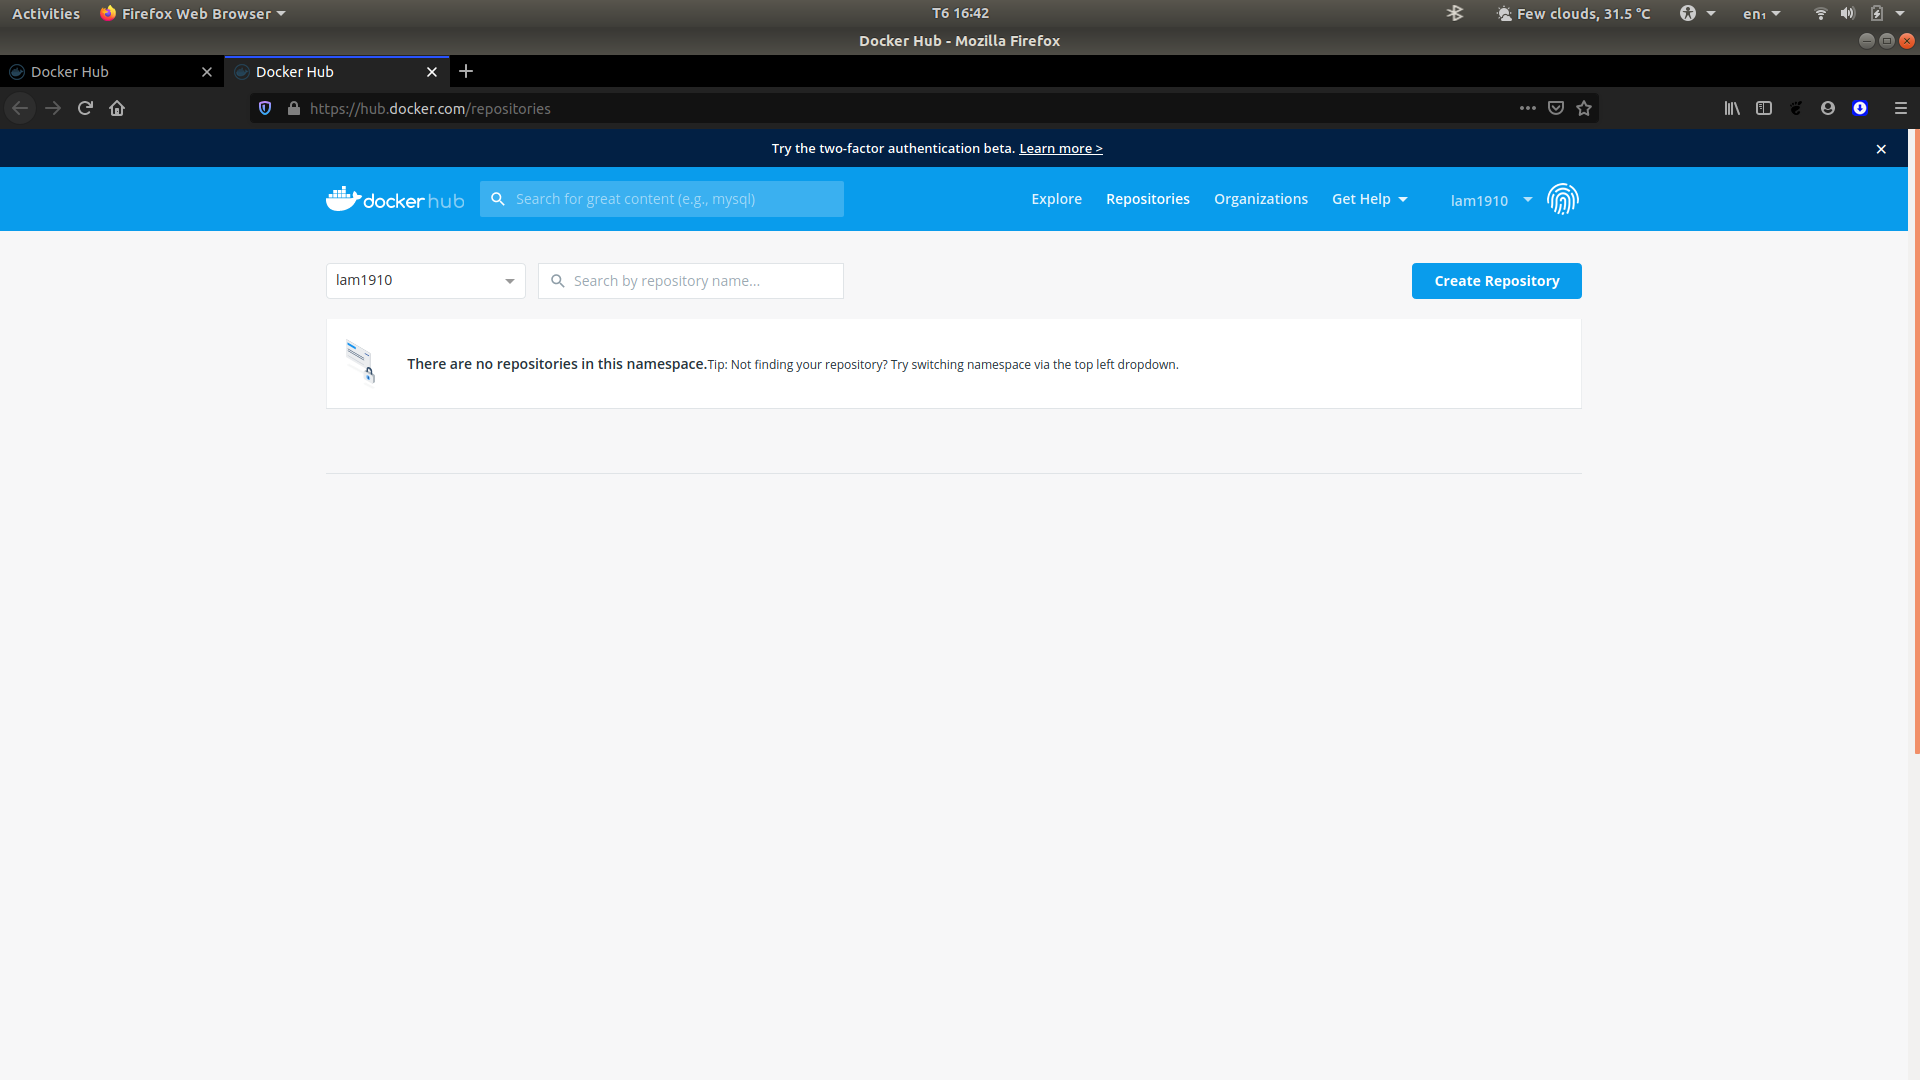
\includegraphics[width=\linewidth]{docker-repo-before.png}
    		\caption{Before pushing anything}
  		\end{subfigure}
  		\begin{subfigure}[b]{\linewidth}
    		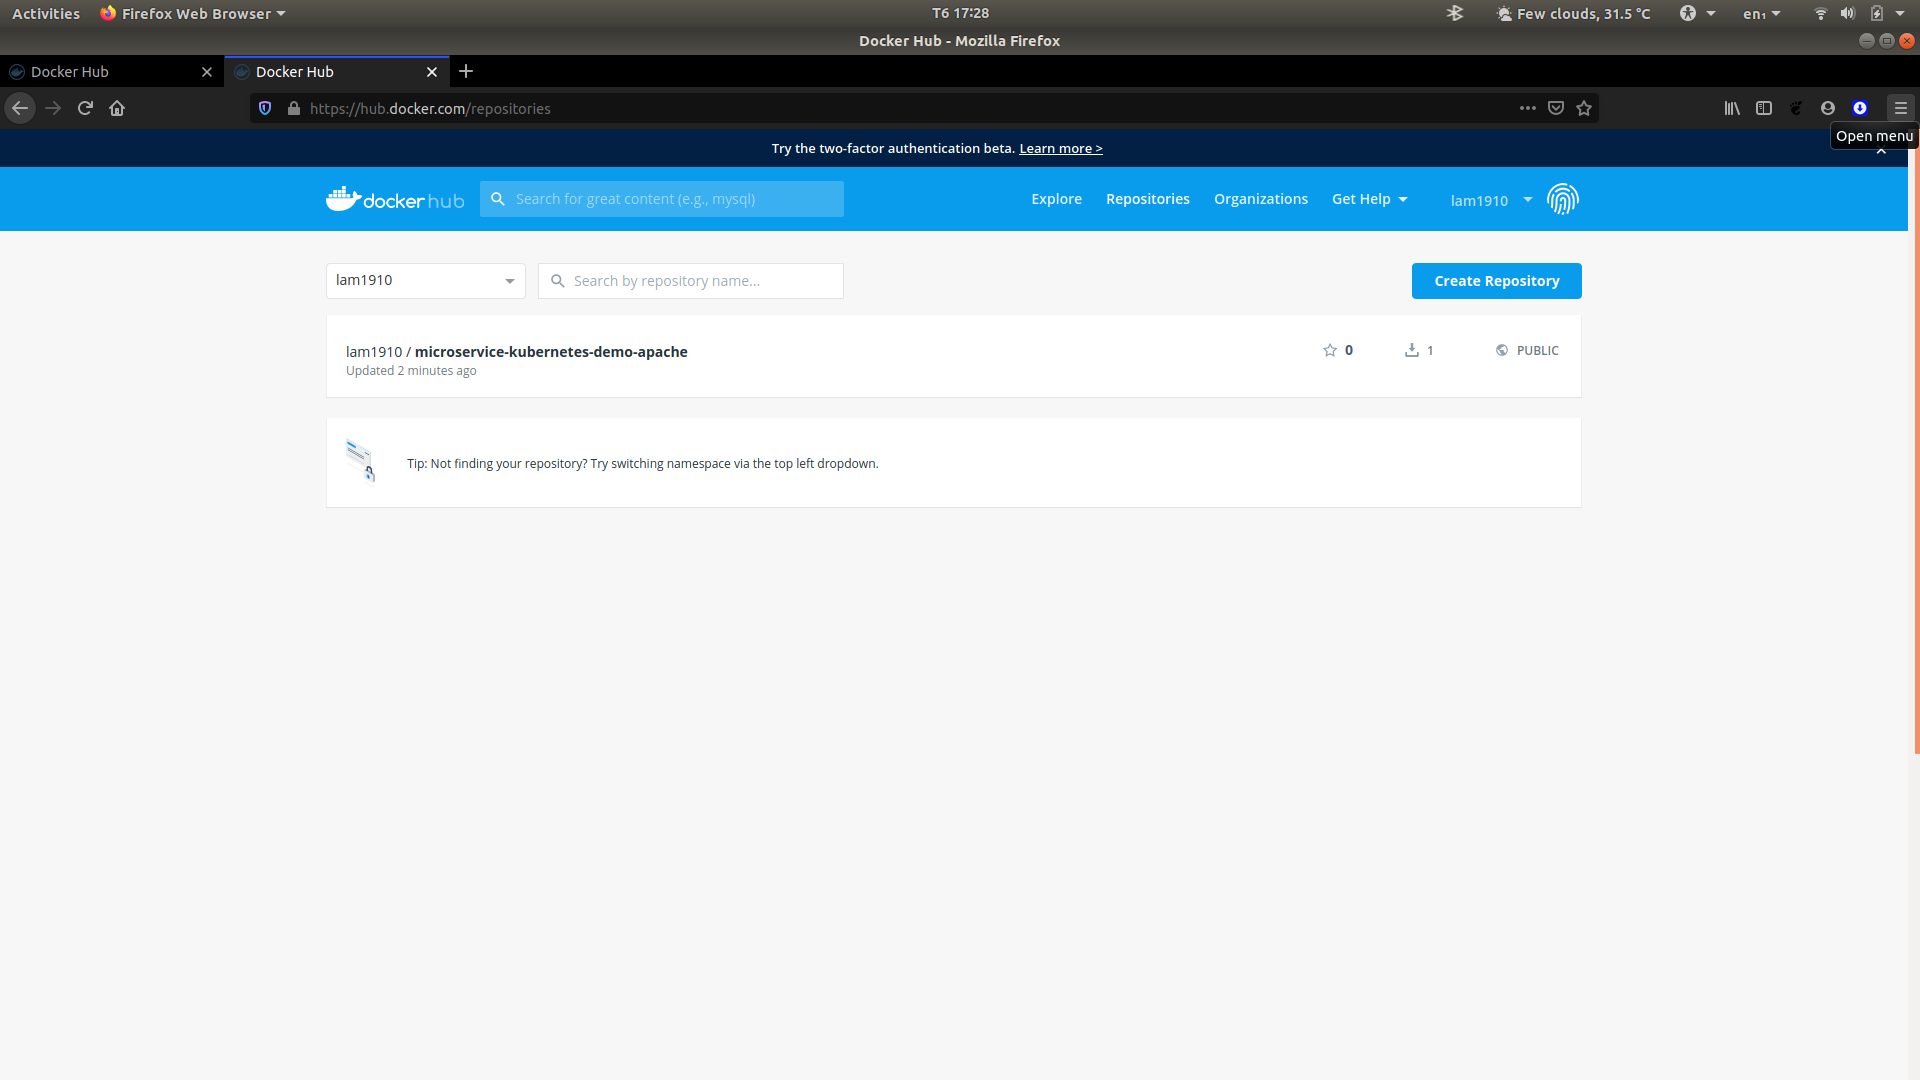
\includegraphics[width=\linewidth]{docker-repo-after.png}
    		\caption{After pushing one service}
  		\end{subfigure}
  		\begin{subfigure}[b]{\linewidth}
    		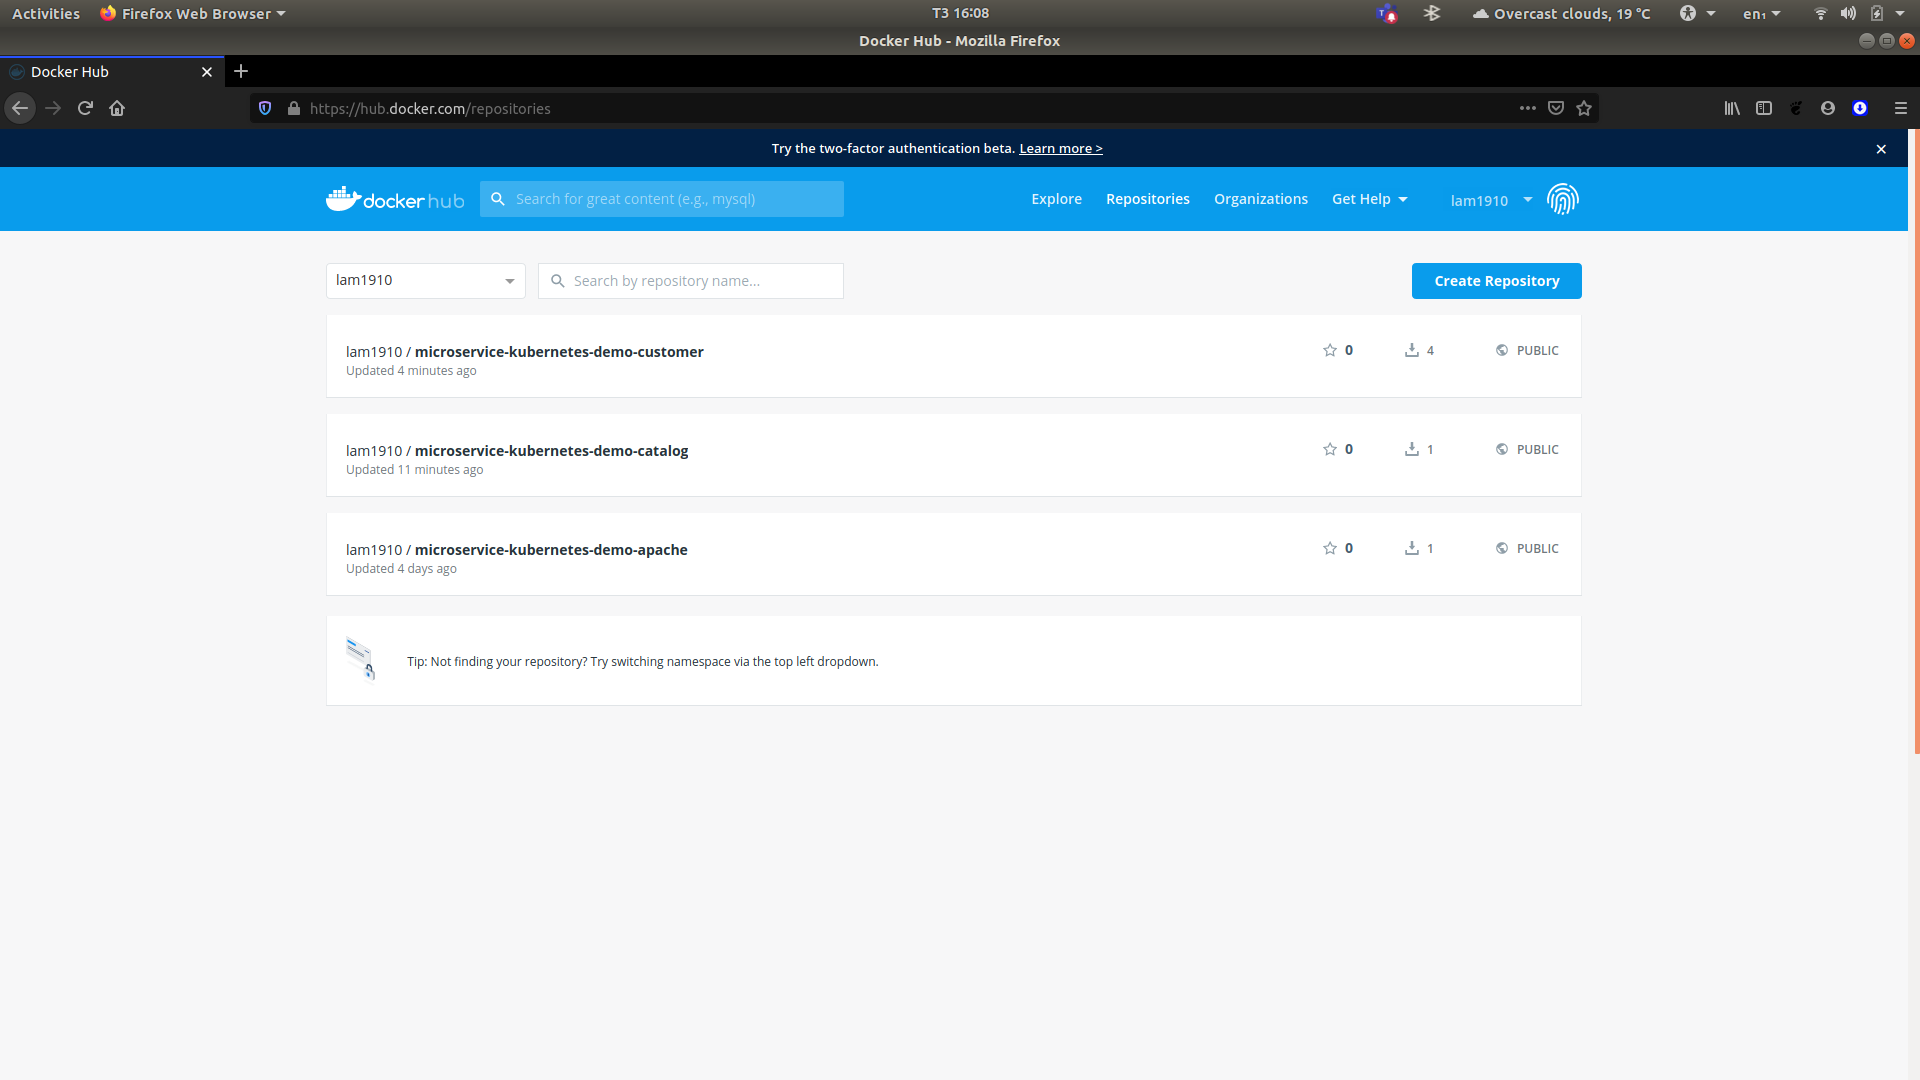
\includegraphics[width=\linewidth]{docker-end-push.png}
    		\caption{After pushing all services}
  		\end{subfigure}
  		\caption{Result from web browser}
  		\label{fig:dockerhubrepo}
	\end{figure}

	\newpage
	\section{Status of Pods}
	\label{sec:stpod}
  	\begin{figure}[h!]
		\centering
  		\begin{subfigure}[b]{0.4\linewidth}
  		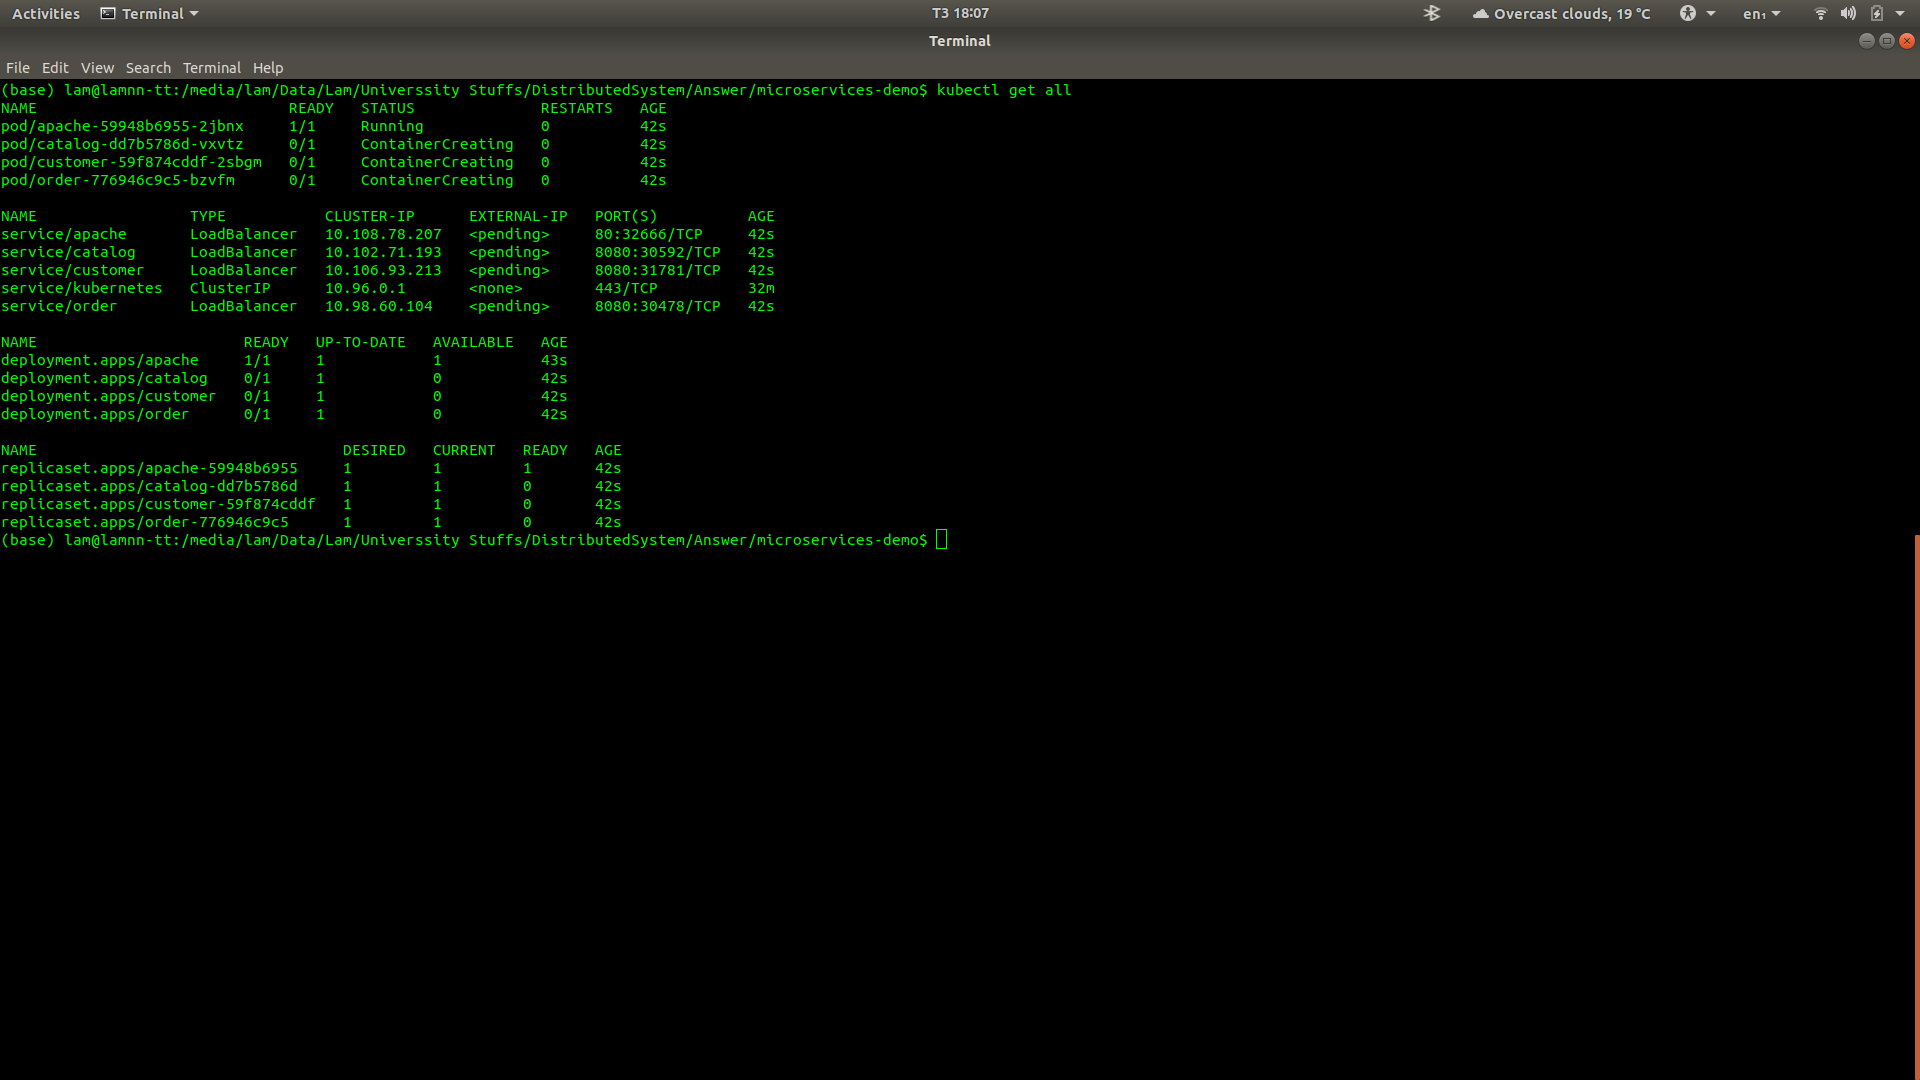
\includegraphics[width=\linewidth]{status-at34.png}
    		\caption{Pods status at second 34th}
  		\end{subfigure}
  		\begin{subfigure}[b]{0.4\linewidth}
    		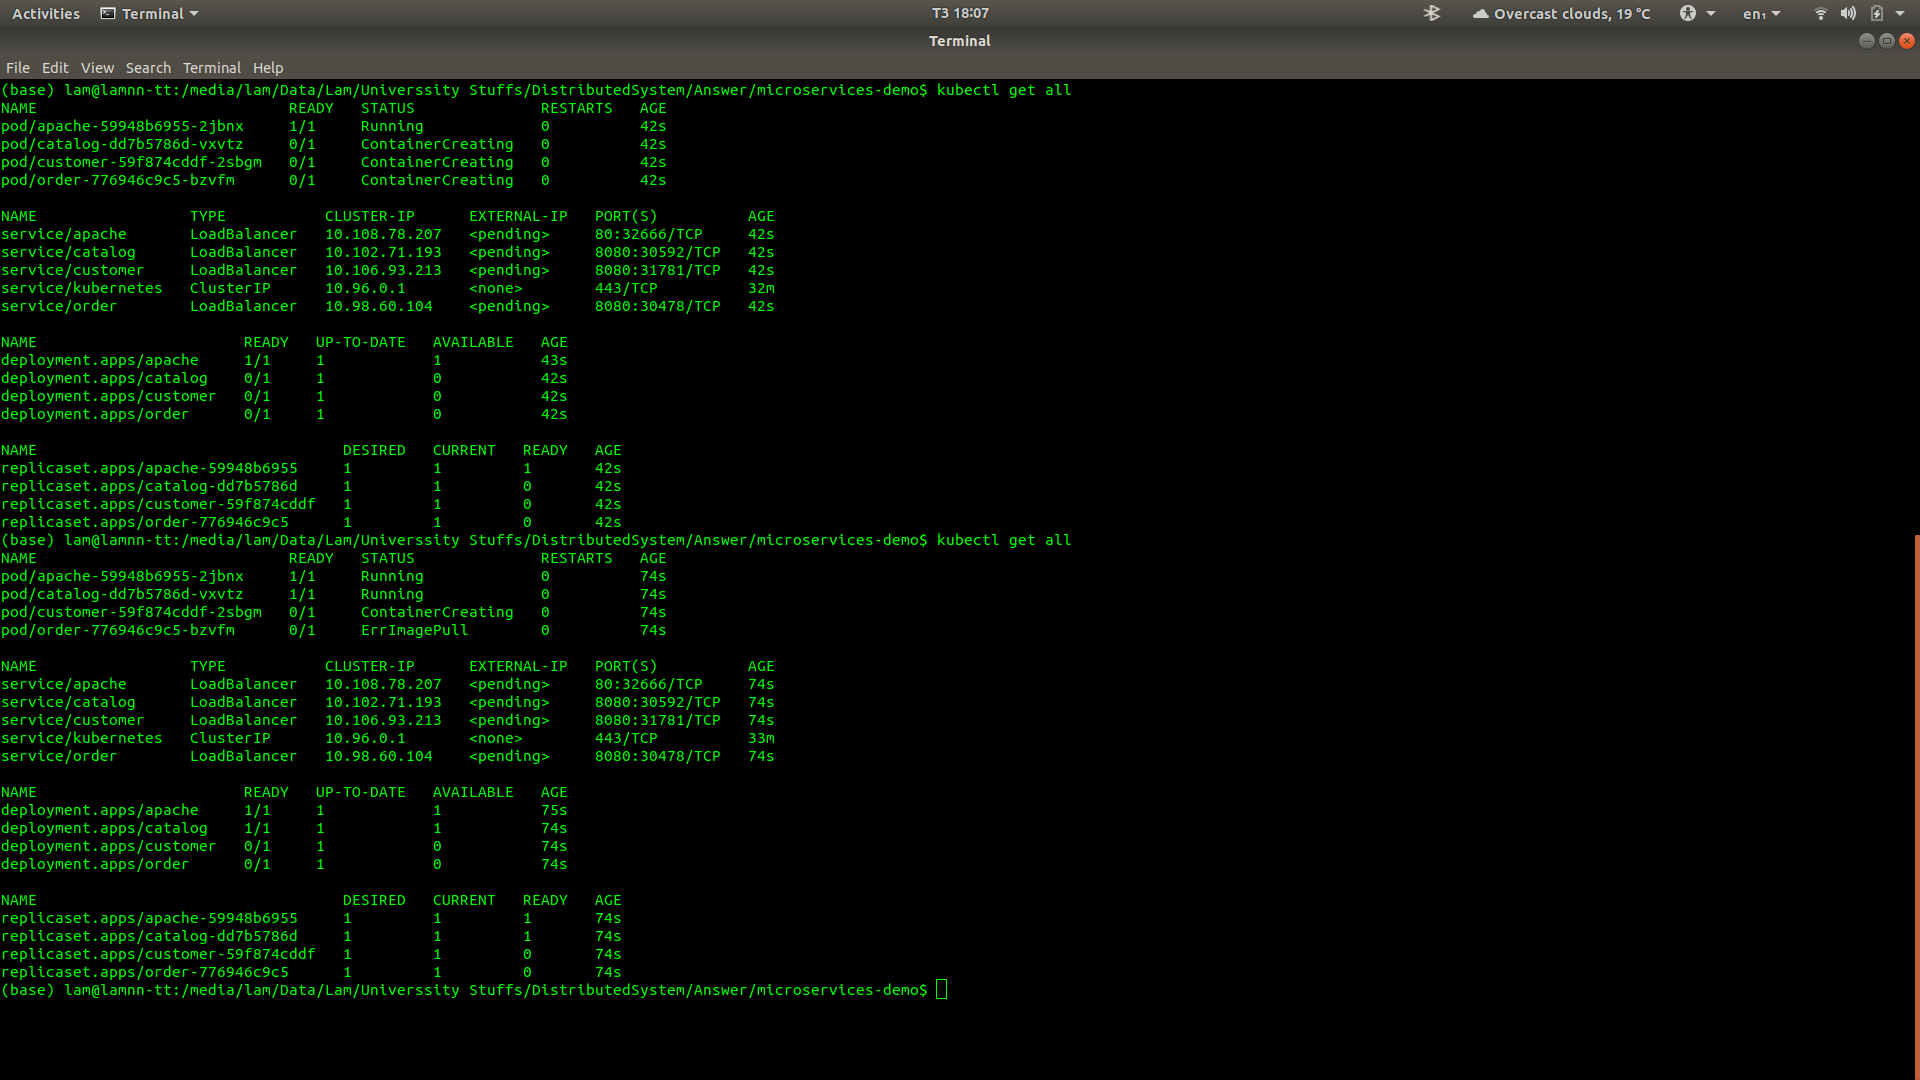
\includegraphics[width=\linewidth]{status-at74.png}
    		\caption{Pods status at second 74th}
  		\end{subfigure}
  		\caption{Status of pods at two time slots}
  		\label{fig:podstat}
	\end{figure}
	The different between two timeframe from \ref{fig:podstat} is that the age of the pods.
	\section{Role of Application Server Glassfish}
	\label{sec:glassfish}
	Glassfish Server is a webserver to deploy web application that was written in java. It uses the Message Queue software as its native JMS provide, providing transparent JMS messaging support.
	\section{Role of the Two JNDIs}
	\label{sec:jndi}
	By making calls to the JNDI API, applications locate resources and other program objects. Each resource object is identified by a unique, people-friendly name, called the JNDI name. A resource object and its JNDI name are bound together by the naming and directory service, which is included with the GlassFish Server. JNDI allows distributed applications to look up services in an abstract, resource-independent way.
	\begin{figure}[h!]
		\centering
  		\begin{subfigure}[b]{0.4\linewidth}
  		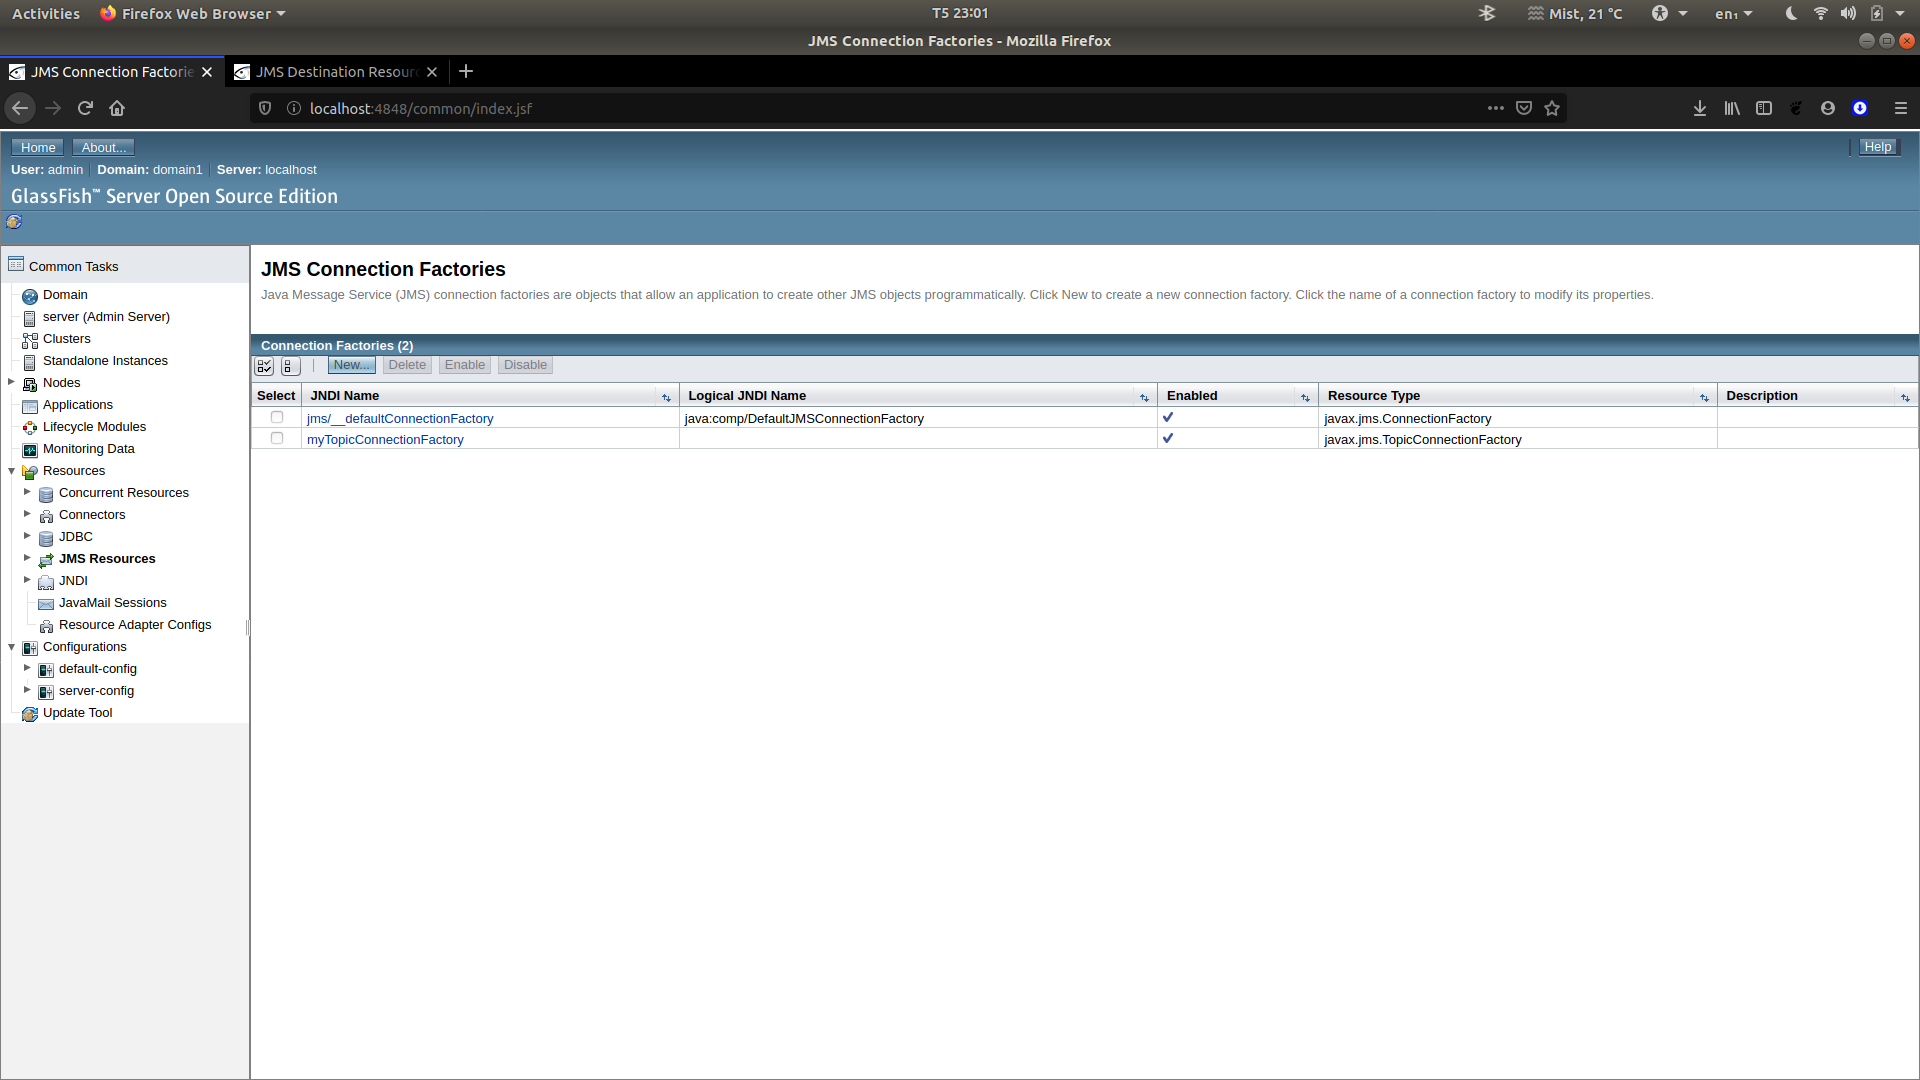
\includegraphics[width=\linewidth]{jndi1.png}
    		\caption{JMS Connection Factories}
  		\end{subfigure}
  		\begin{subfigure}[b]{0.4\linewidth}
    		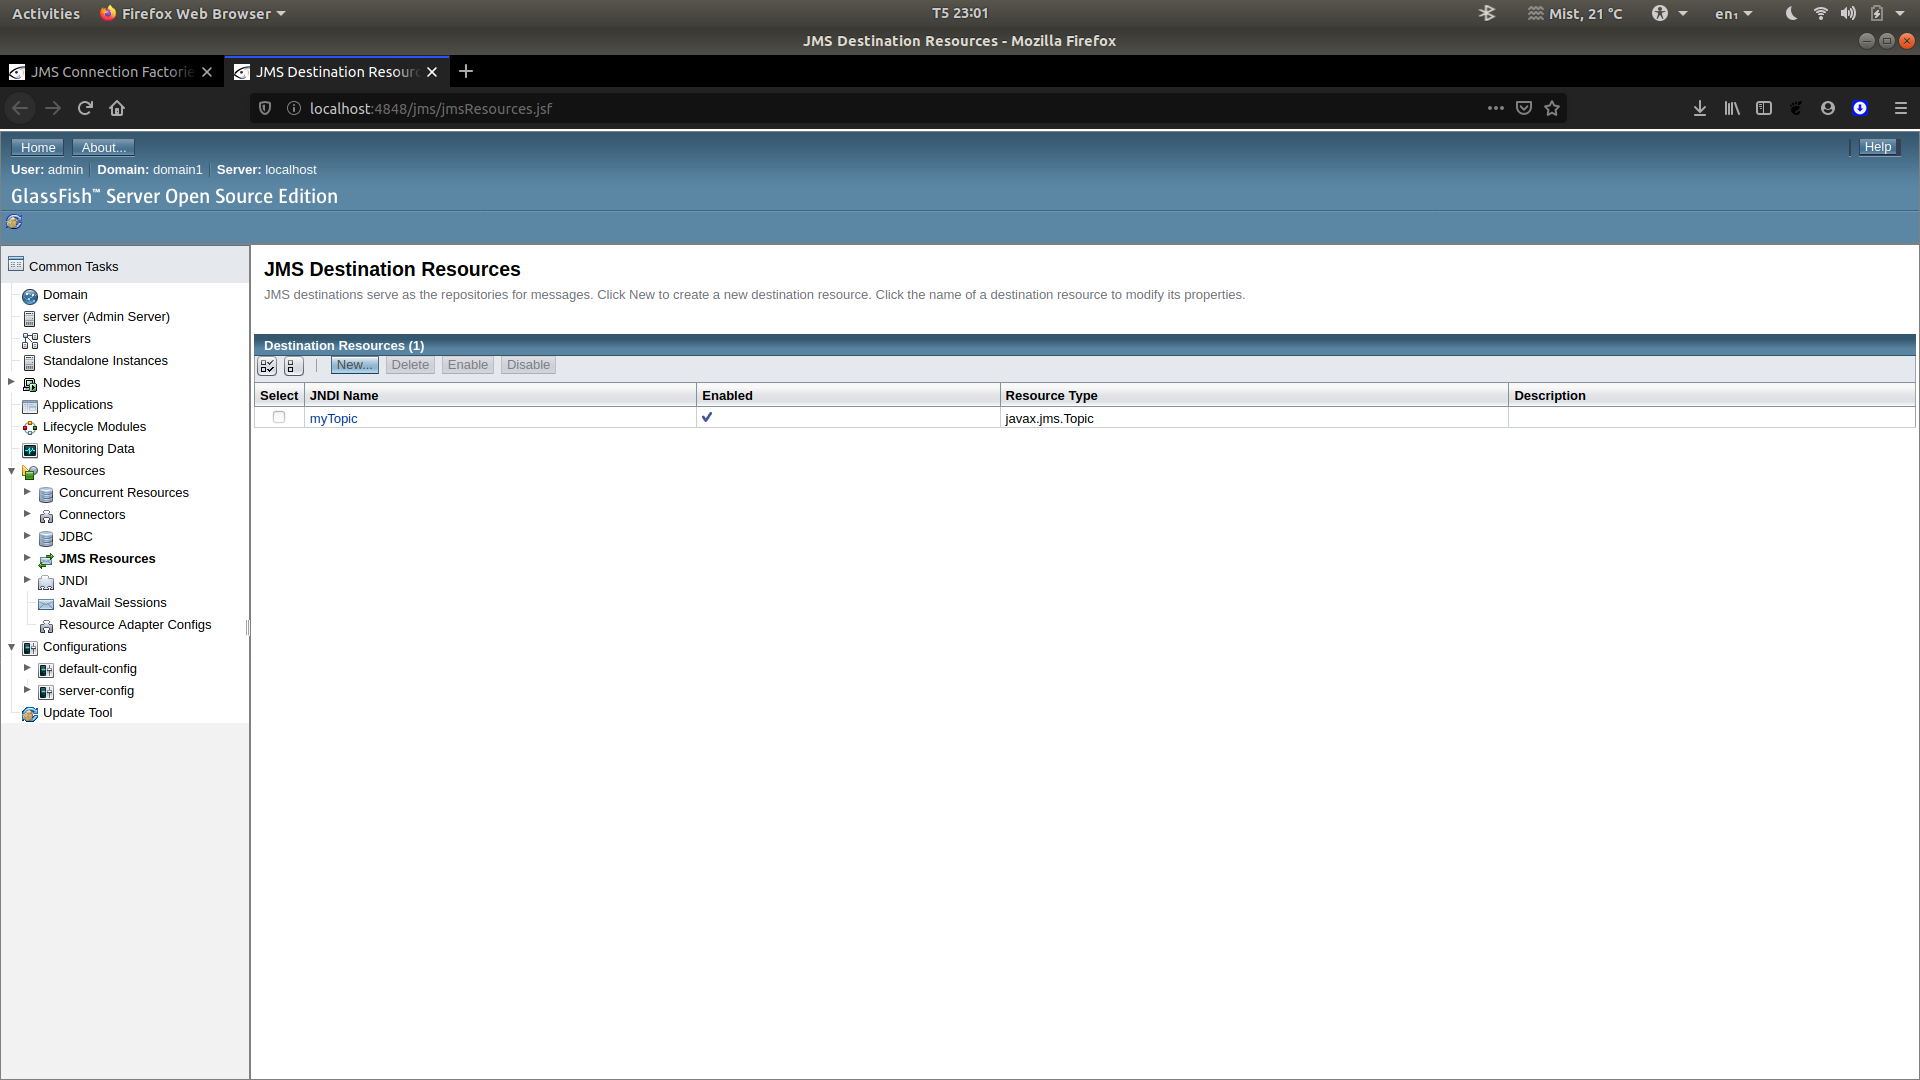
\includegraphics[width=\linewidth]{jndi2.png}
    		\caption{JMS Destination Resources}
  		\end{subfigure}
  		\caption{JNDIs}
  		\label{fig:jndi}
	\end{figure}
	\section{The Message Passing Method of Sender and Receiver Explaination}
	\label{sec:mespassexpl}
	\begin{figure}[h!]
		\centering
  		\begin{subfigure}[b]{0.4\linewidth}
  		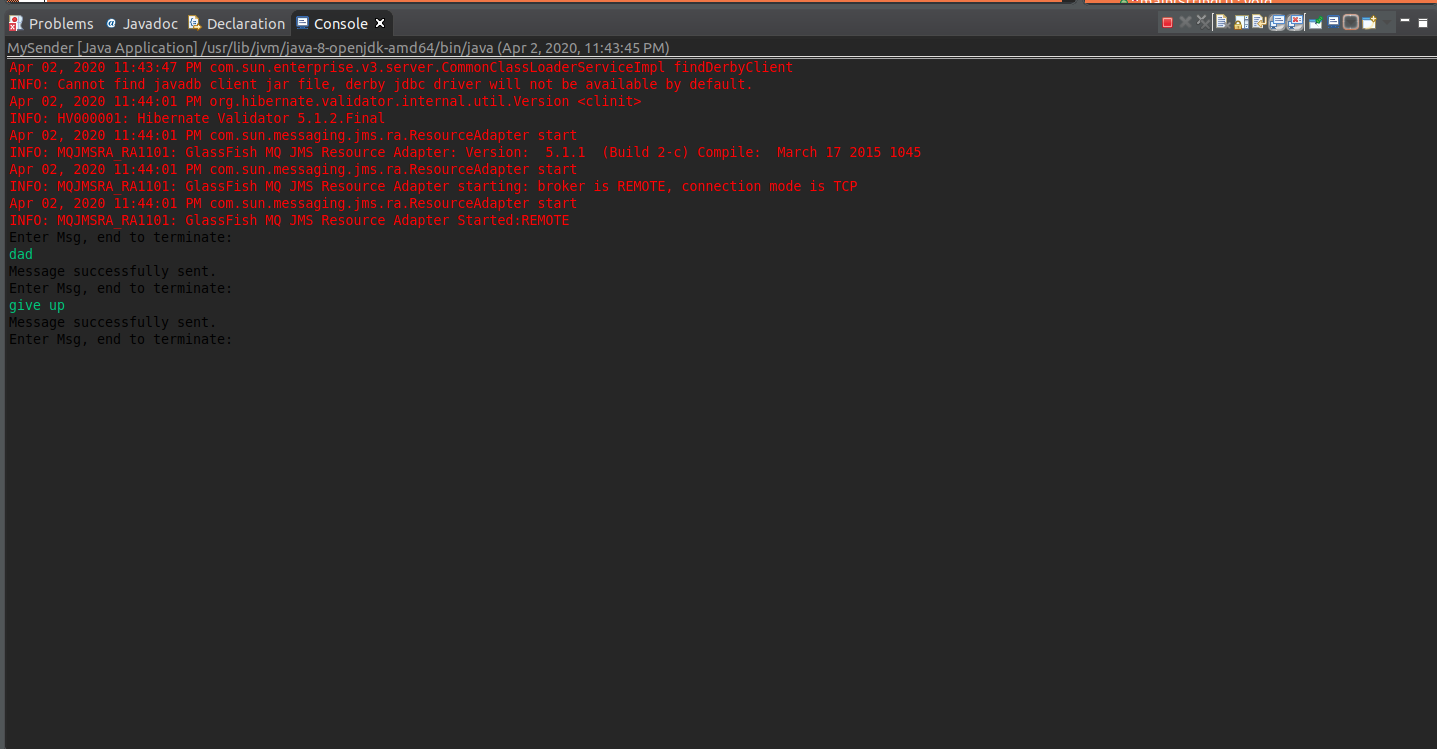
\includegraphics[width=\linewidth]{sender-res.png}
    		\caption{Sender}
  		\end{subfigure}
  		\begin{subfigure}[b]{0.4\linewidth}
    		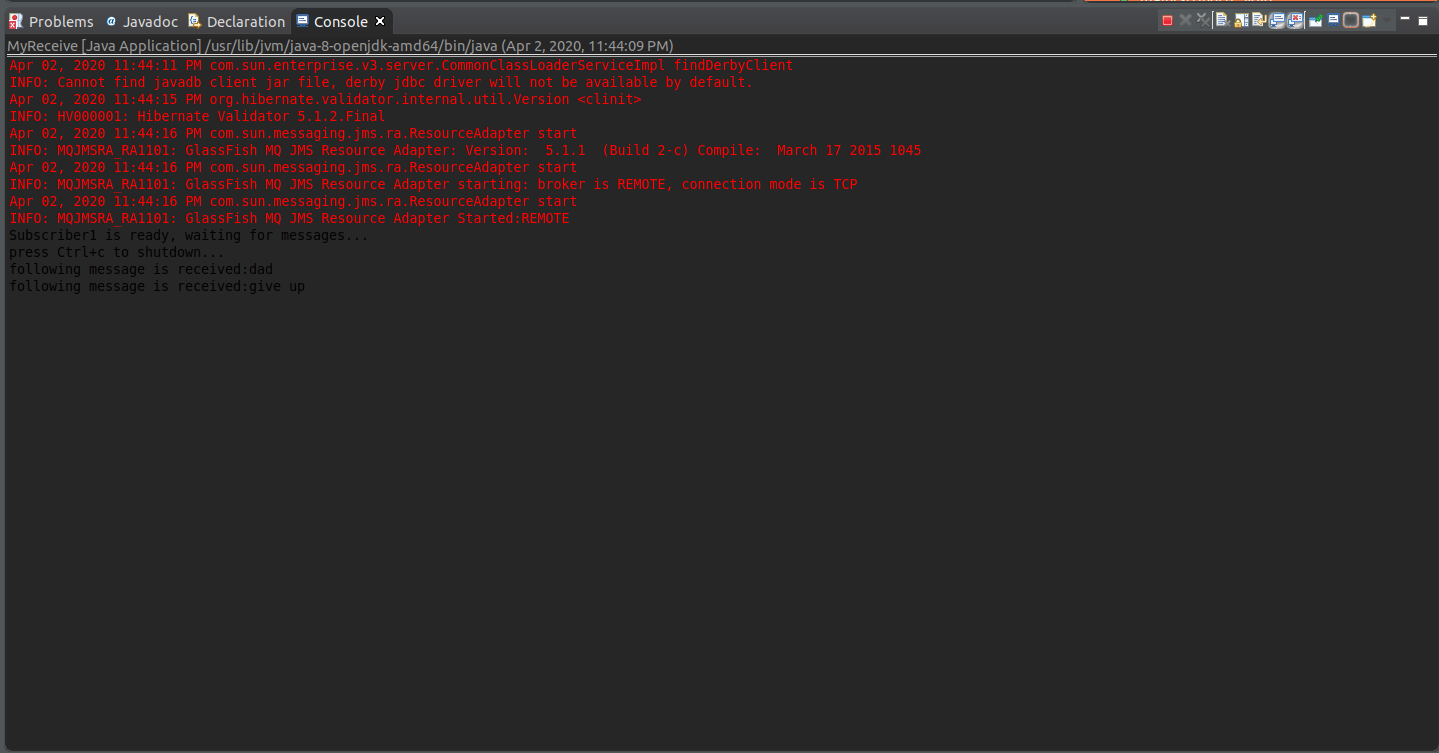
\includegraphics[width=\linewidth]{receiver-res.png}
    		\caption{Receiver}
  		\end{subfigure}
  		\caption{Result of running MySender and MyReceiver}
  		\label{fig:jndi}
	\end{figure}
	Explanation:
	\begin{enumerate}
		\item The Sender get the topic object named ''myTopic''
		\item It creates a publisher to register that event
		\item It creates buffer to store user input and publish the message to subscribers of event ''myTopic''
		\item In regard to the Receiver, it subscriber to ''myTopic'' and be able to receive the Sender’s message
		\item When the Sender publishes the message, since the Receiver has already subscribed to that event and get that message
	\end{enumerate}
	\section{Compare the JMS and DDS}
	\begin{tabular}{|c|c|}
	\hline 
	JMS & DDS \\ 
	\hline 
	Java Messaging Service & Data Distributed Service \\ 
	\hline 
	Used for sending messages & DDS is networking middleware \\ between two or more clients & that simplifies complex \\&network programming. \\&It implements a \\& publish/subscribe model  \\&for sending and receiving data, \\&events, and commands among nodes. \\
	\hline 
	Centralized & Decentralized \\ 
	\hline 
	Allows the communication between & Automatically handles all\\ different components of  & aspects of message delivery \\ a distribute application &\\
	\hline 
	\end{tabular} 
		
\end{document}